\section{Results}
\label{sec:results}

We have implemented and tested our methods on 26 different real-world datasets.
The vast majority of datasets studied were sourced from Outlier Detection Datasets (ODDS), which provided clear labels for normal and anomalous behavior.
We examine the effectiveness of our methods by their ability to identify these outliers.

Figure~\ref{results:datasets} shows % TODO
We chose to use so many different real world datasets to ensure that our methods could generalize to many target audiences.

\begin{figure*}[!t]
\centering
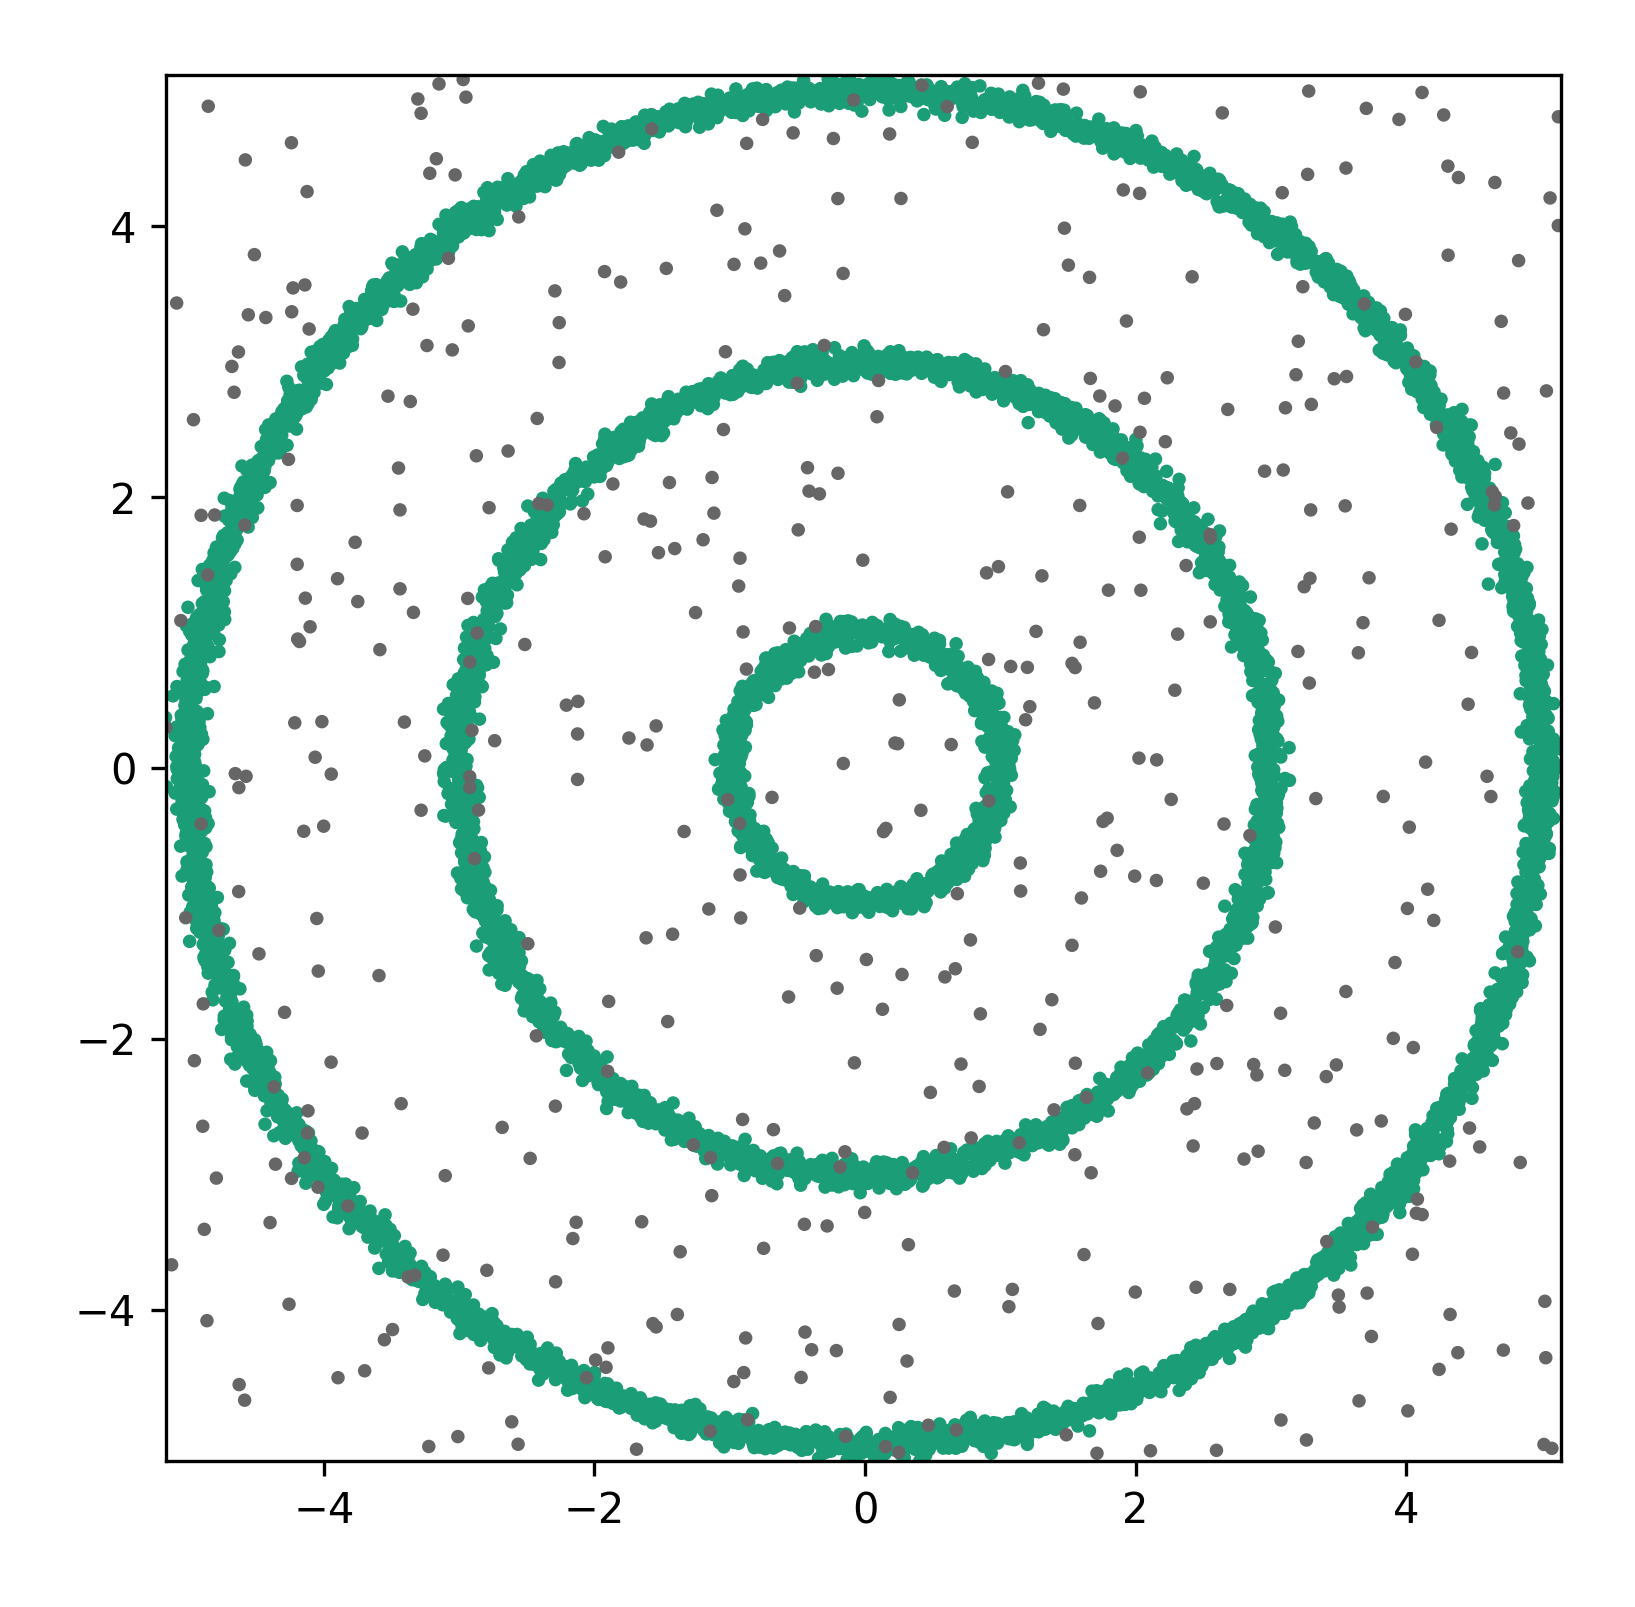
\includegraphics[width=2.5in]{static/bullseye.png}
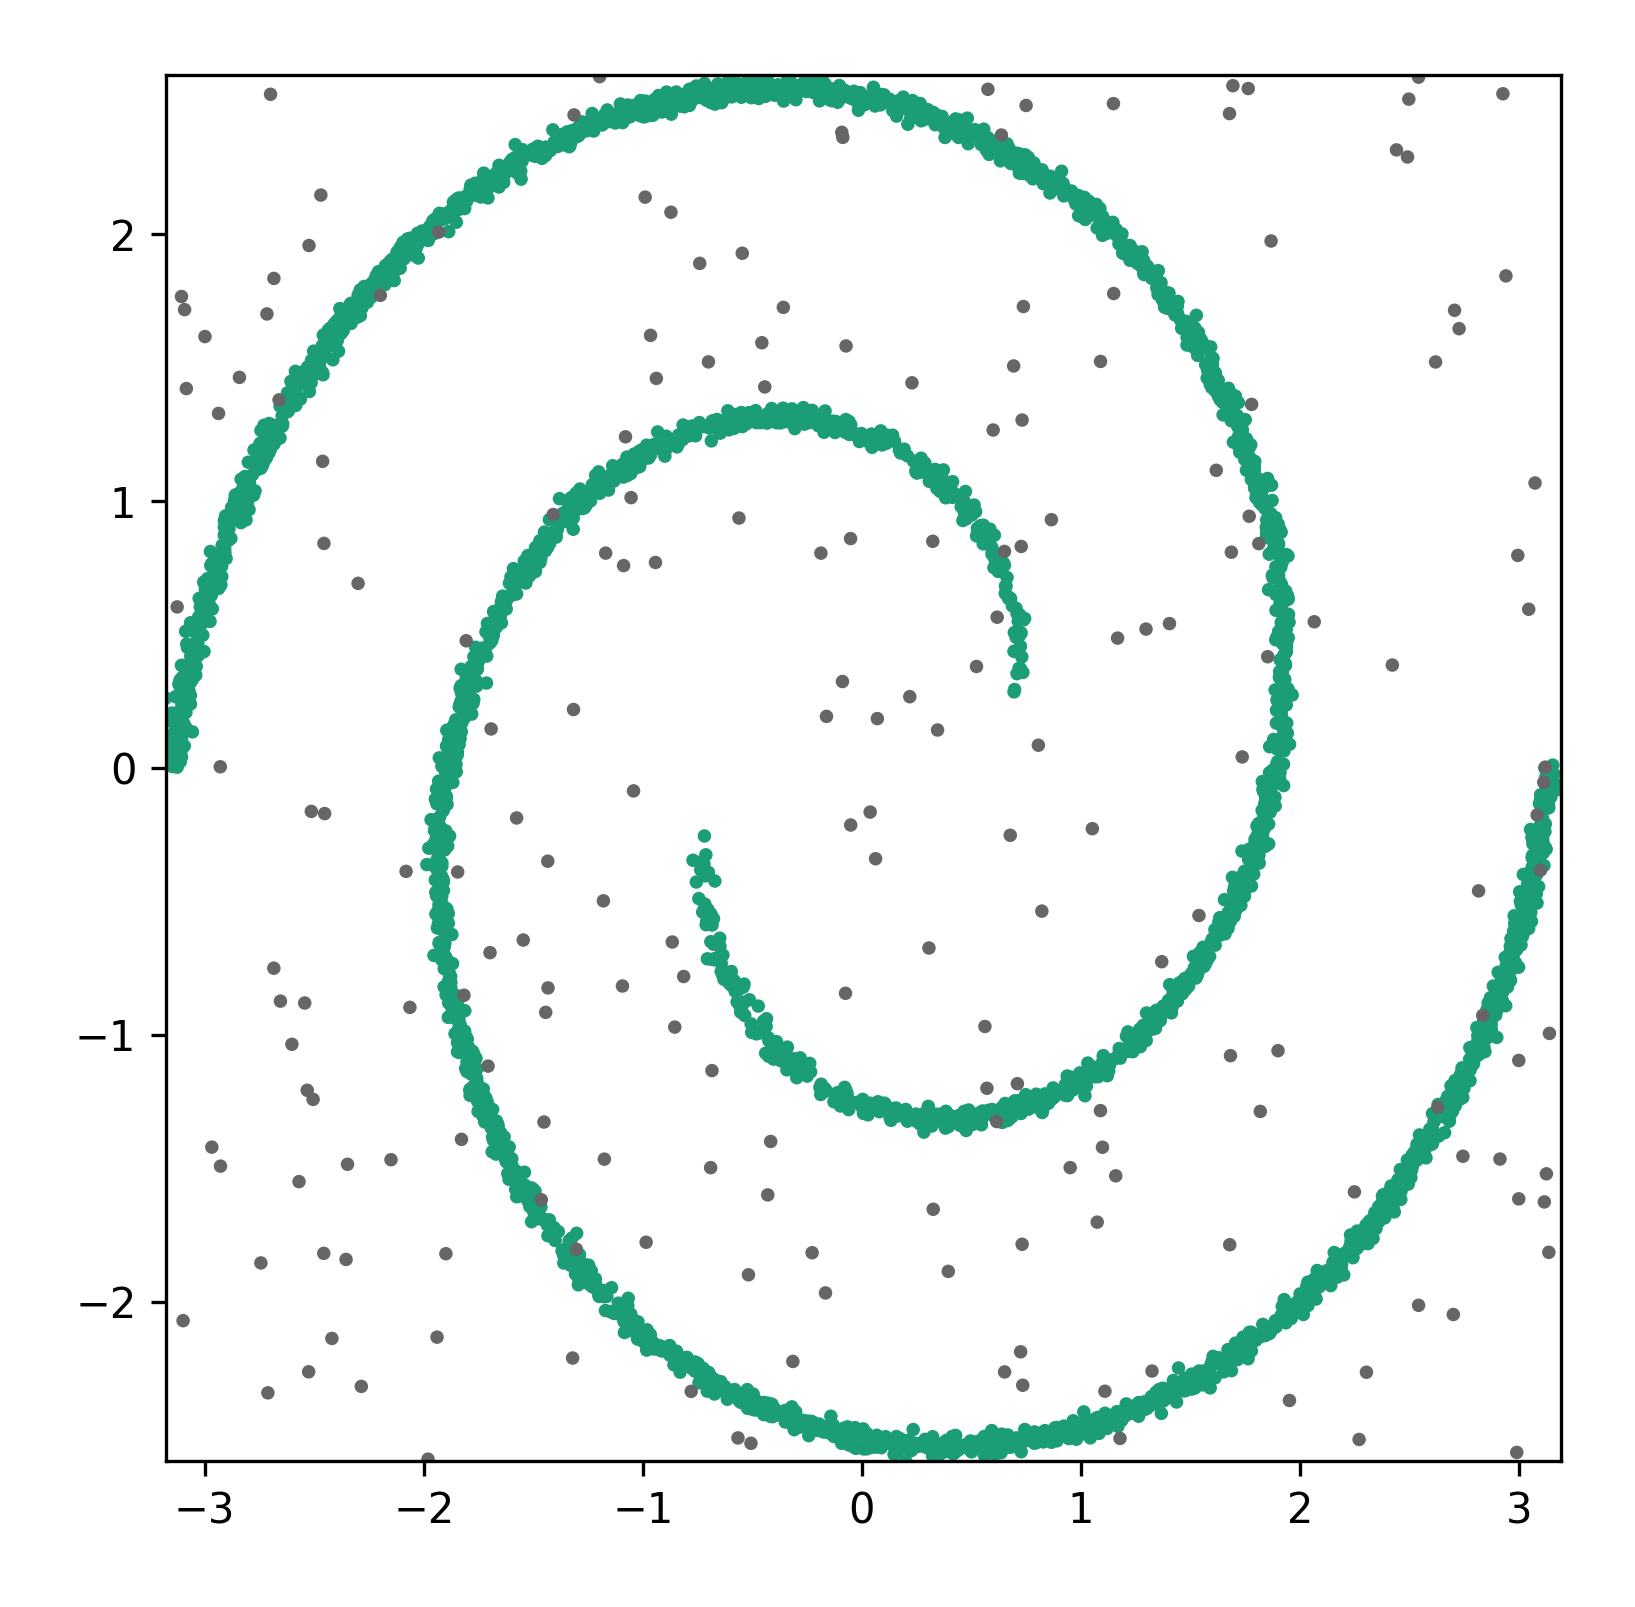
\includegraphics[width=2.5in]{static/spiral.png}
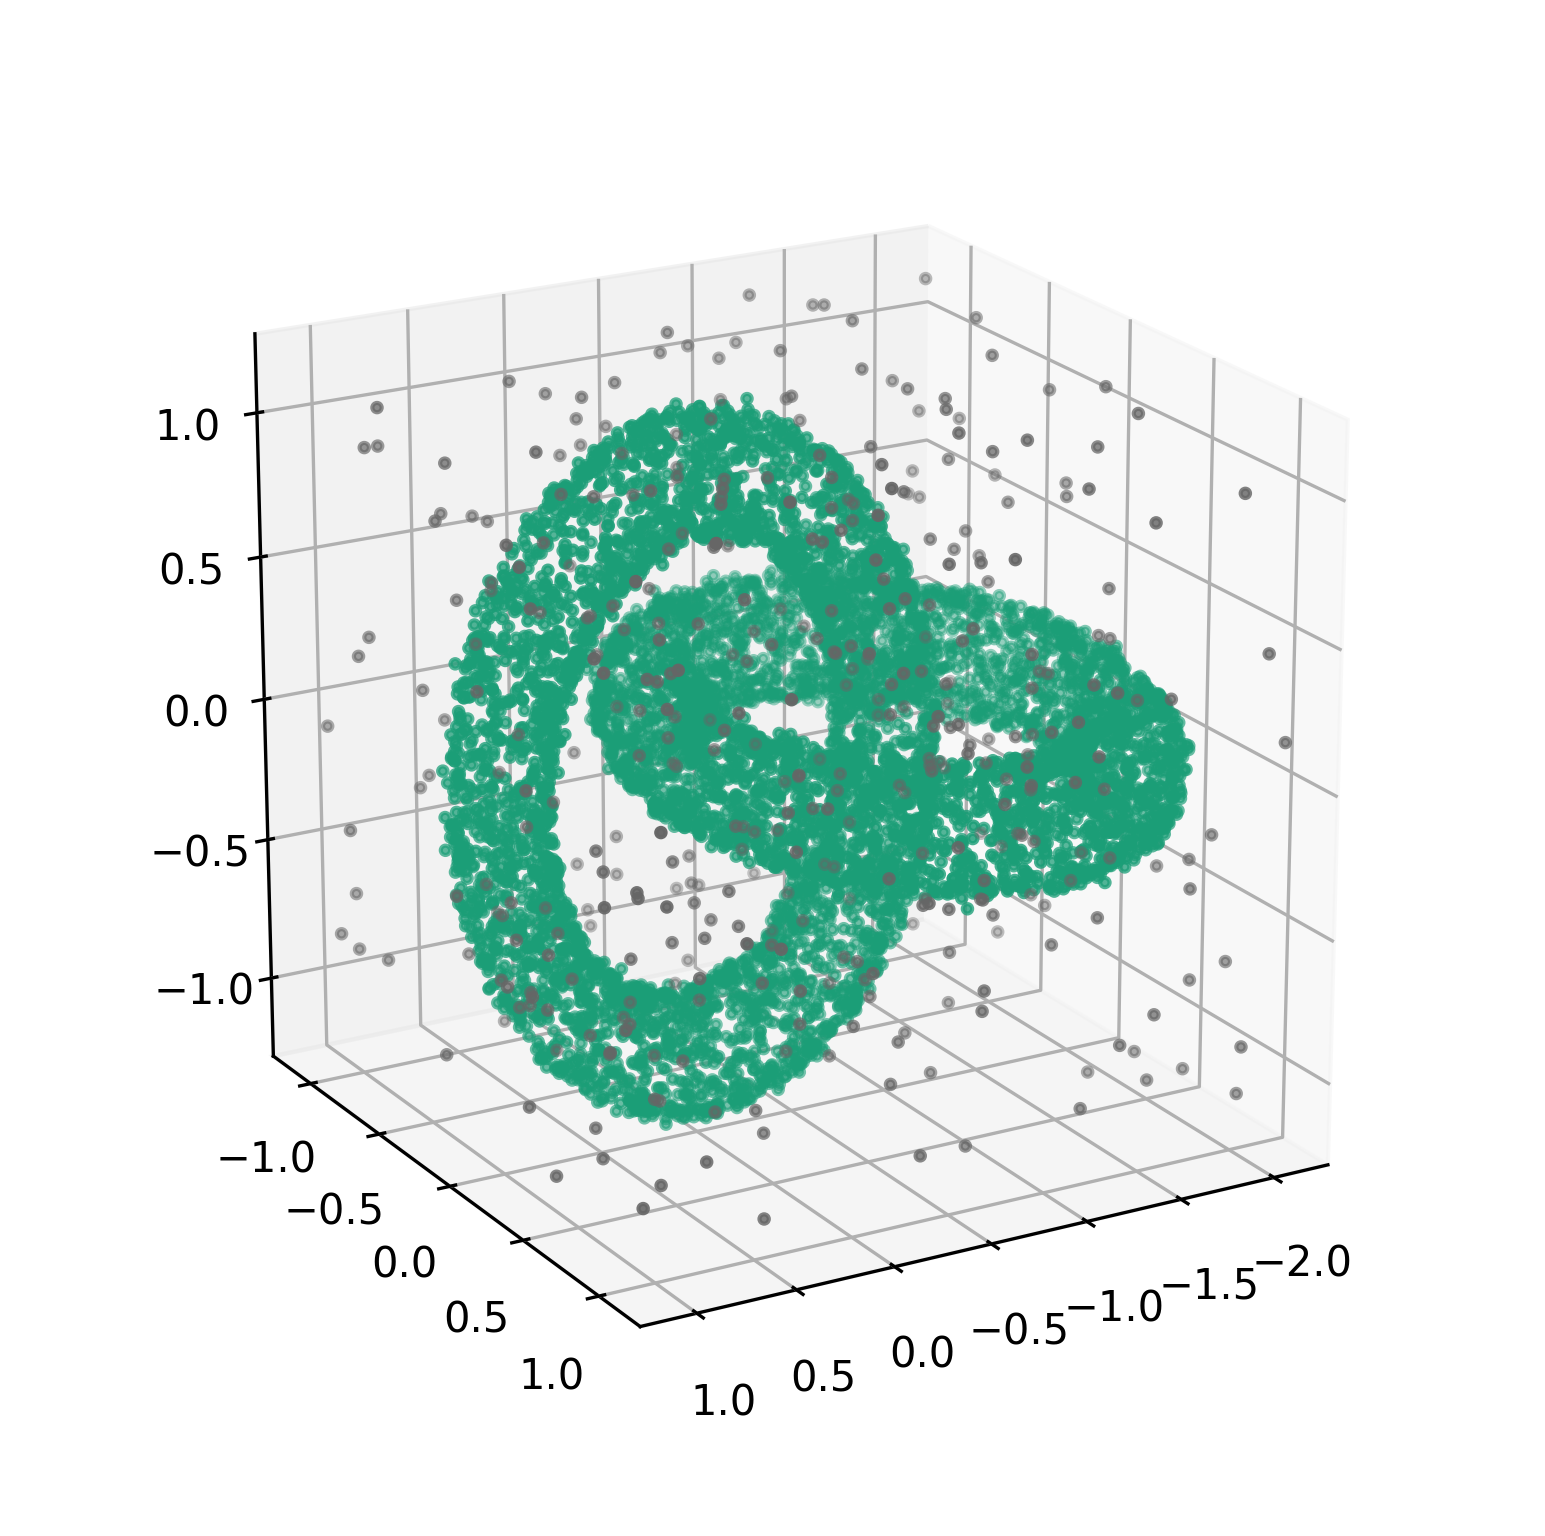
\includegraphics[width=3in]{static/interlocking_tori.png}
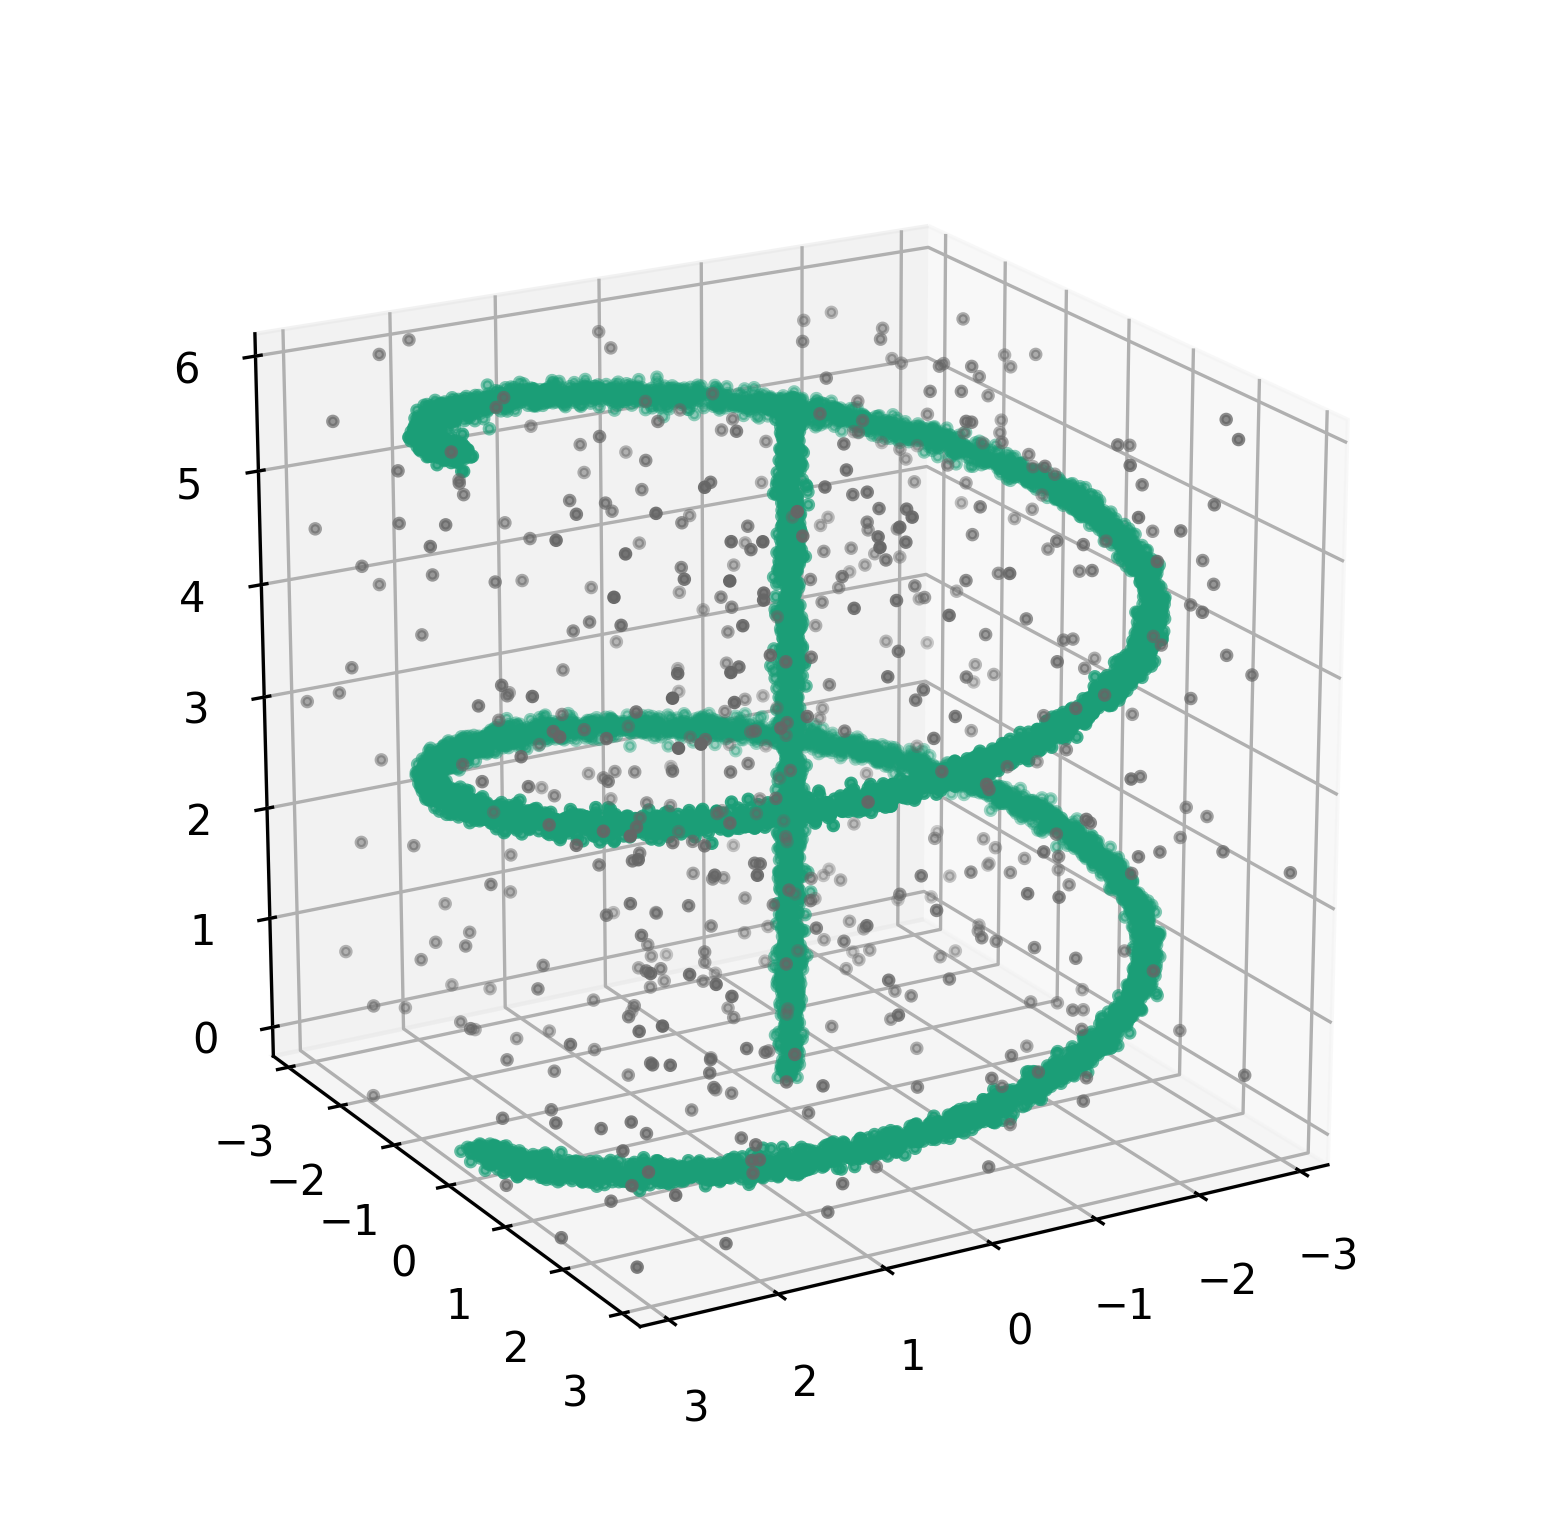
\includegraphics[width=3in]{static/skewer.png}
\caption{The Bullseye (top-left), Spiral (top-right), Interlocking Tori (bottom-left) and Skewer (bottom-left) datasets.}
\label{results:datasets}
\end{figure*}

For each dataset, we clustered using Manhattan, Euclidean, and Cosine distance functions.
Additionally, for this work, we allowed CLAM to cluster down until the manifold had thoroughly shattered.
We then iterated over all depths to compute the area under the ROC-Curve.

After computing anomalousness scores, we normalized each metric to a $[0, 1]$ range.
For each dataset, we present a confusion matrix, a ROC curve, and the area under the ROC curve for a sample of optimal depths. 
To demonstrate our methods are not overly-sensitive to depth we present all metrics in a 5-depth wide window.

Table~\ref{results:table} lists % TODO

Figures~\ref{results:histograms:kth_nearest}, \ref{results:histograms:hierarchical}, \ref{results:histograms:outrank}, and \ref{results:histograms:k_neighborhood} shows histograms of measured anomalousness for points in each dataset for each method used.
Higher values of anomalousness indicate higher confidence that the point is an anomaly.

\begin{table*}[!t]
\renewcommand{\arraystretch}{1.3}
\caption{Anomaly Detection performance on the synthetic datasets.}
\label{results:table}
\centering
\begin{tabular}{|c|c|c|c|c|c|c|c|c|}
\hline
 & \multicolumn{2}{c|}{\textbf{Bullseye}} & \multicolumn{2}{c|}{\textbf{Spiral}} & \multicolumn{2}{c|}{\textbf{Interlocking}} & \multicolumn{2}{c|}{\textbf{Skewer}} \\
  & \multicolumn{2}{c|}{\textbf{ }} & \multicolumn{2}{c|}{\textbf{ }} & \multicolumn{2}{c|}{\textbf{Tori}} & \multicolumn{2}{c|}{\textbf{ }} \\
\hline
 & \bfseries TPR & \bfseries TNR & \bfseries TPR & \bfseries TNR & \bfseries TPR & \bfseries TNR & \bfseries TPR & \bfseries TNR \\
\hline
\bfseries k$^{th}$-nearest Distances & 1.000 & 0.979 & 1.000 & 0.020 & 1.000 & 0.979 & 1.000 & 0.979 \\
\hline
\bfseries Hierarchical Sparseness & 0.985 & 0.940 & 1.000 & 0.969 & 0.992 & 0.961 & 1.000 & 0.967 \\
\hline
\bfseries Outrank Algorithm & 0.998 & 0.990 & 1.000 & 0.987 & 1.000 & 0.989 & 1.000 & 0.989 \\
\hline
\bfseries k-Neighborhood Size & 0.996 & 0.990 & 0.990 & 0.984 & 0.761 & 0.986 & 0.975 & 0.983 \\
\hline
\end{tabular}
\end{table*}

\begin{figure*}[!t]
\centering
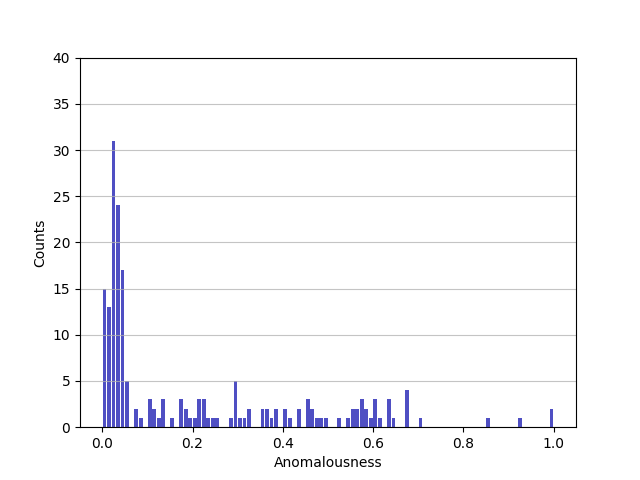
\includegraphics[width=2.5in]{static/bullseye_kth_nearest.png}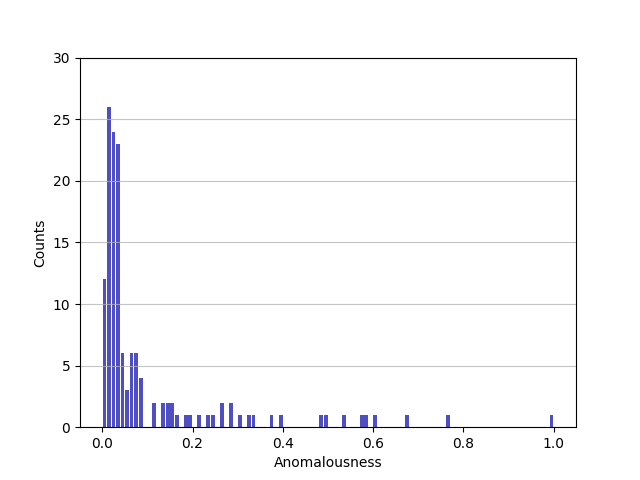
\includegraphics[width=2.5in]{static/spiral_kth_nearest.png}

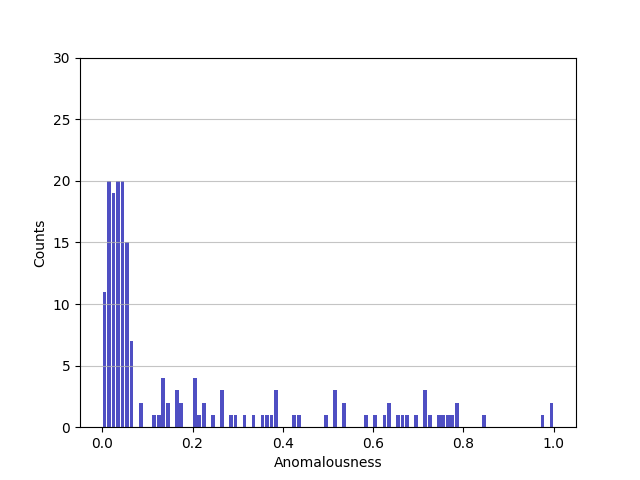
\includegraphics[width=2.5in]{static/interlocking_tori_kth_nearest.png}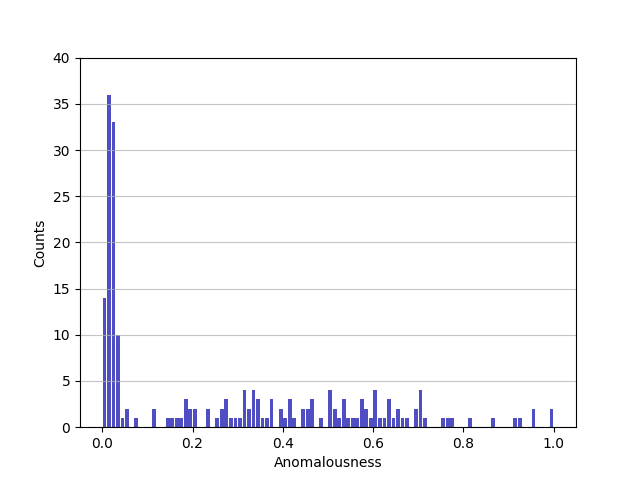
\includegraphics[width=2.5in]{static/skewer_kth_nearest.png}

\caption{
Measures of anomalousness using the k$^{th}$-nearest Distances method on the Bullseye (top-left), Spiral (top-right), Interlocking-Tori (bottom-left), and the Skewer (bottom-right) datasets.
}

\label{results:histograms:kth_nearest}
\end{figure*}

% 1.7in seems to be the right width for four-across images
\begin{figure*}[!t]
\centering
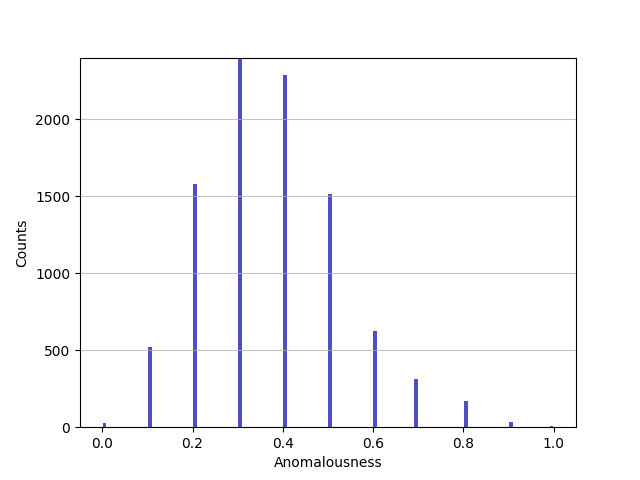
\includegraphics[width=1.7in]{static/bullseye_hierarchical.png}
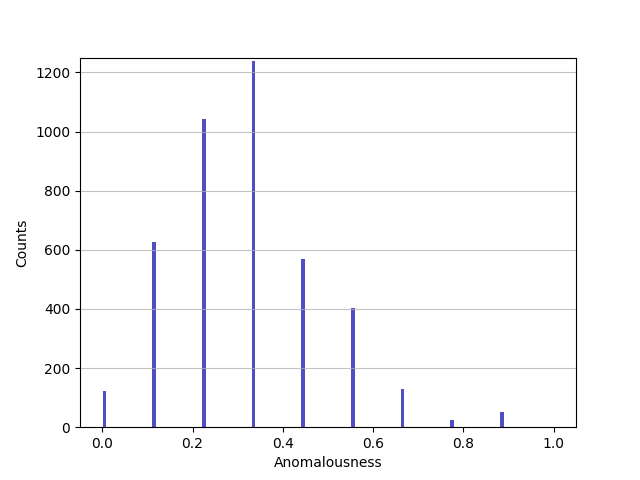
\includegraphics[width=1.7in]{static/spiral_hierarchical.png}
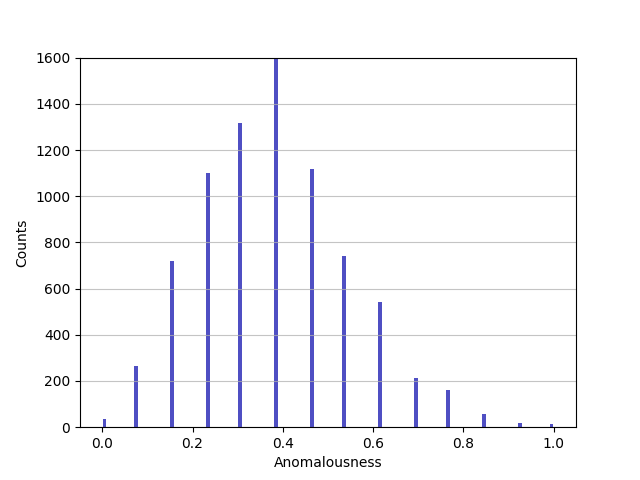
\includegraphics[width=1.7in]{static/interlocking_tori_hierarchical.png}
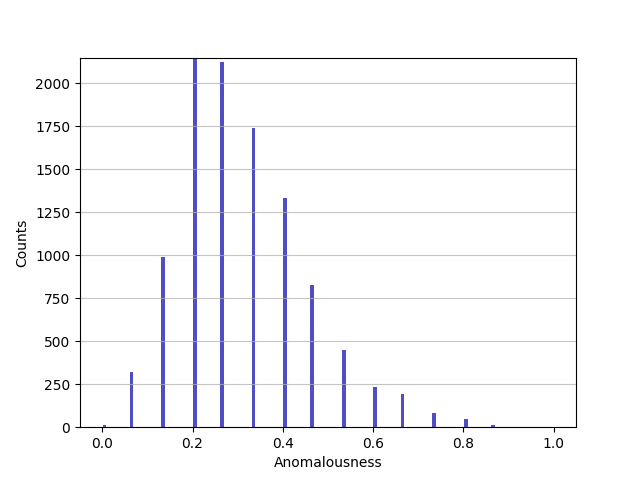
\includegraphics[width=1.7in]{static/skewer_hierarchical.png}

\caption{
Measures of anomalousness using the Hierarchical Sparseness method on the Bullseye (top-left), Spiral (top-right), Interlocking-Tori (bottom-left), and the Skewer (bottom-right) datasets.
}

\label{results:histograms:hierarchical}
\end{figure*}


% 1.7in seems to be the right width for four-across images
\begin{figure*}[!t]
\centering
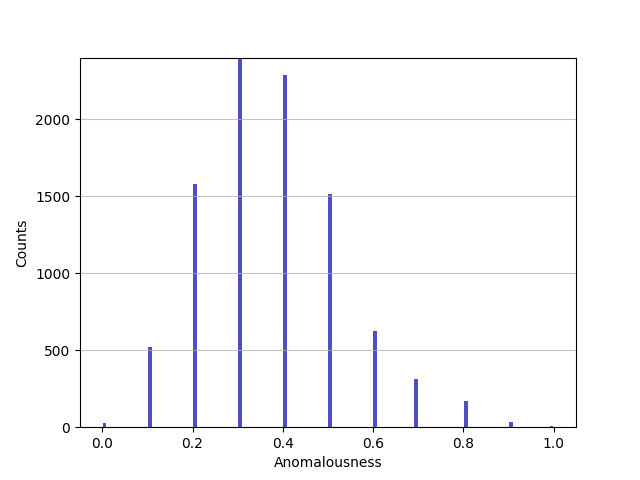
\includegraphics[width=1.7in]{static/bullseye_hierarchical.png}
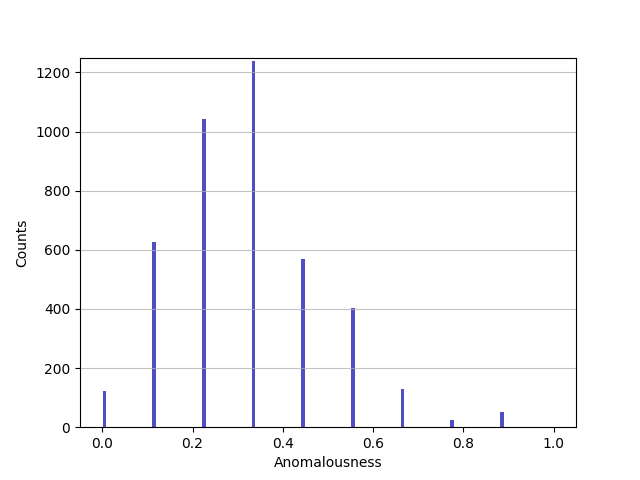
\includegraphics[width=1.7in]{static/spiral_hierarchical.png}
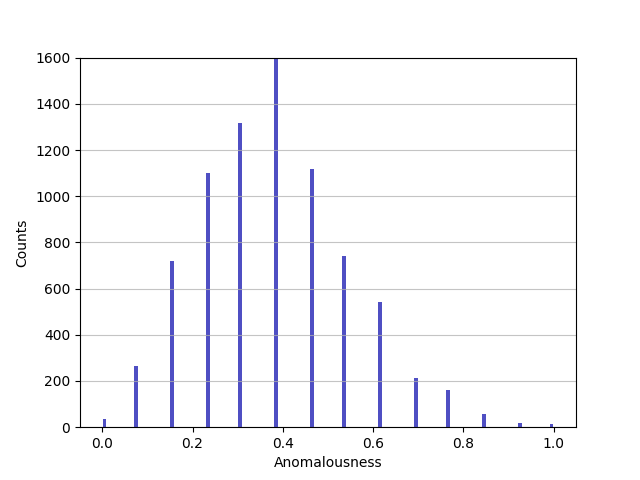
\includegraphics[width=1.7in]{static/interlocking_tori_hierarchical.png}
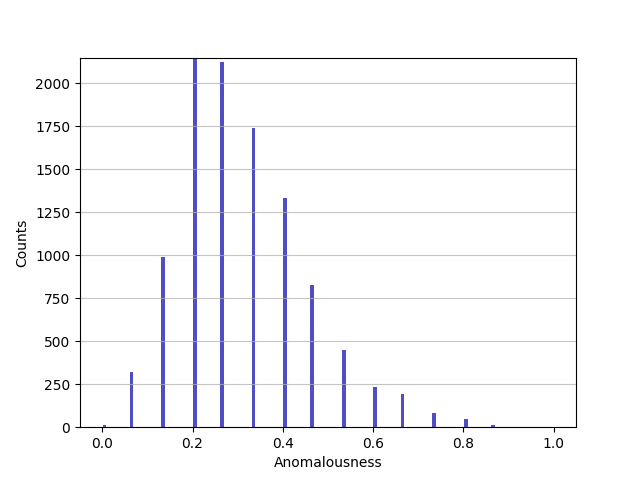
\includegraphics[width=1.7in]{static/skewer_hierarchical.png}
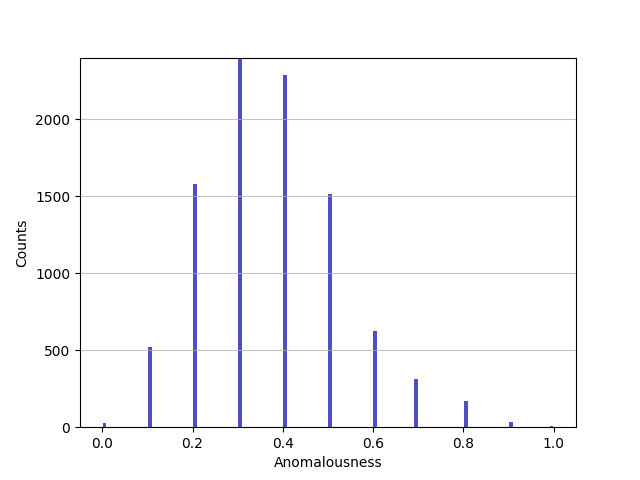
\includegraphics[width=1.7in]{static/bullseye_hierarchical.png}
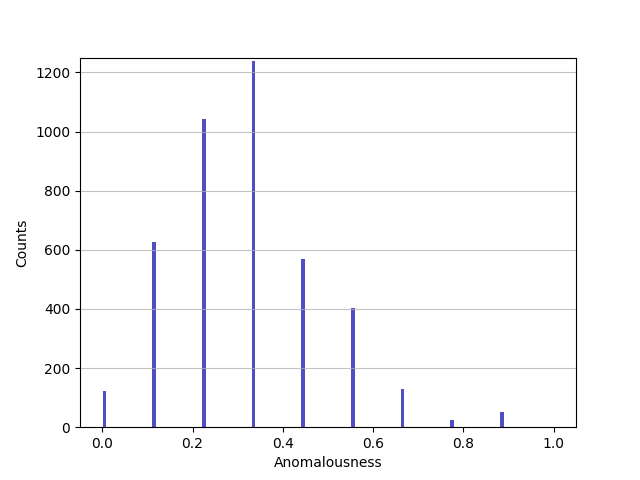
\includegraphics[width=1.7in]{static/spiral_hierarchical.png}
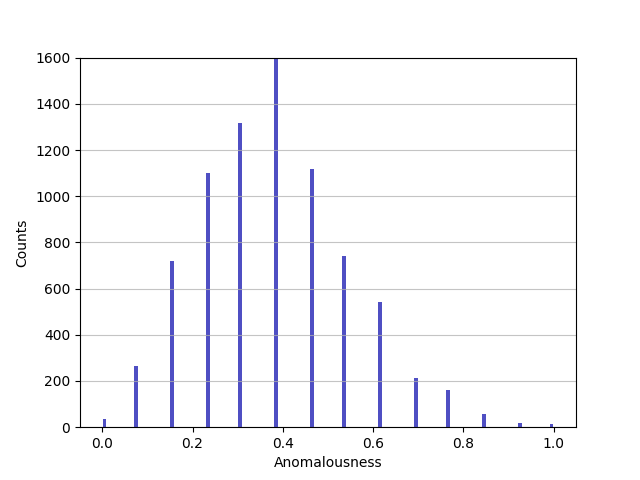
\includegraphics[width=1.7in]{static/interlocking_tori_hierarchical.png}
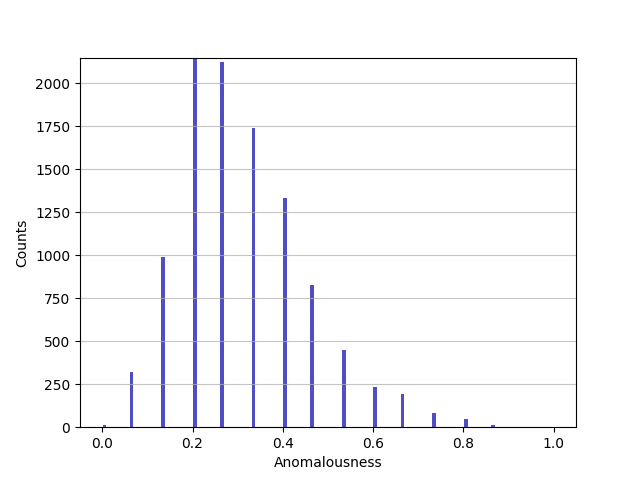
\includegraphics[width=1.7in]{static/skewer_hierarchical.png}
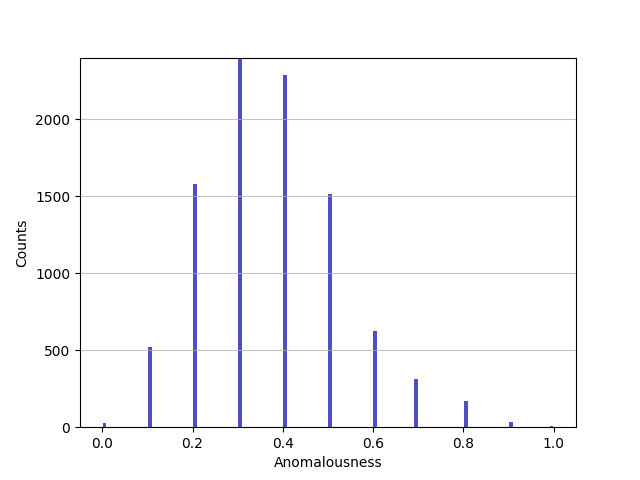
\includegraphics[width=1.7in]{static/bullseye_hierarchical.png}
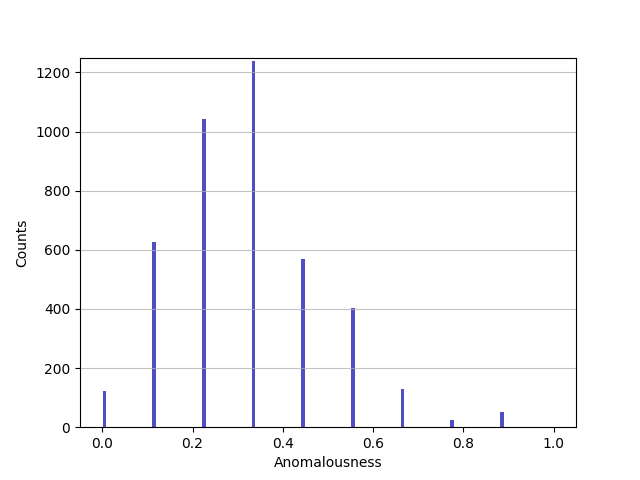
\includegraphics[width=1.7in]{static/spiral_hierarchical.png}
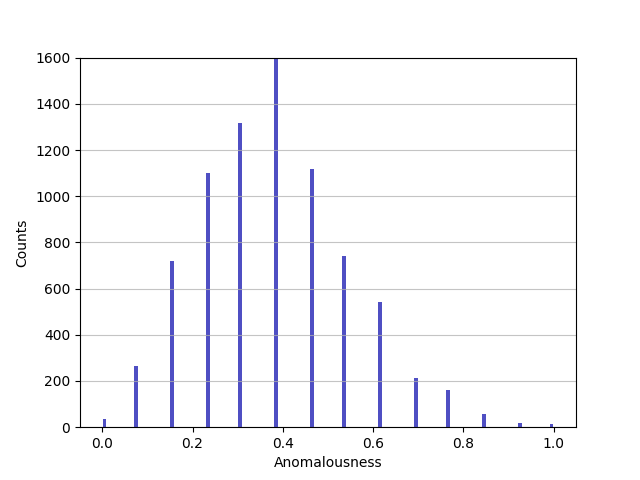
\includegraphics[width=1.7in]{static/interlocking_tori_hierarchical.png}
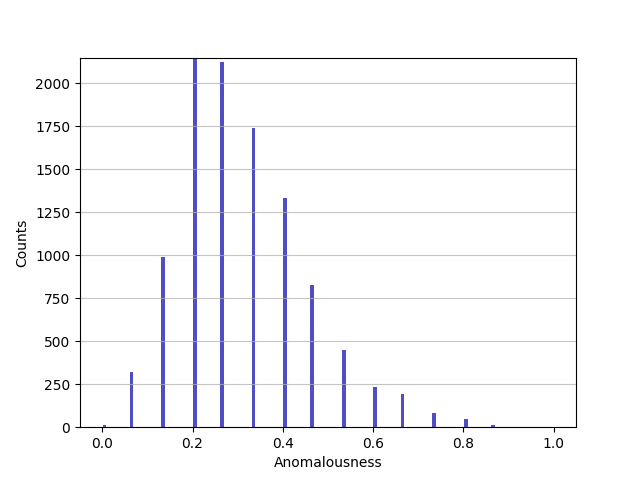
\includegraphics[width=1.7in]{static/skewer_hierarchical.png}

\caption{
Example of a grid of regular-sized images.
}

\label{results:histograms:example}
\end{figure*}


\begin{figure*}[!t]
\centering
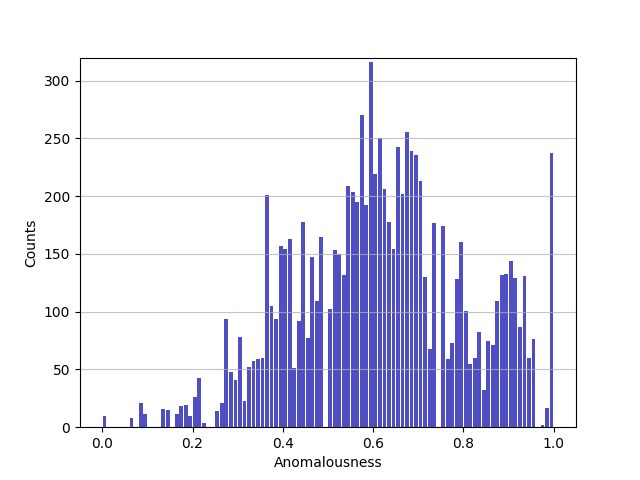
\includegraphics[width=2.5in]{static/bullseye_outrank.png}
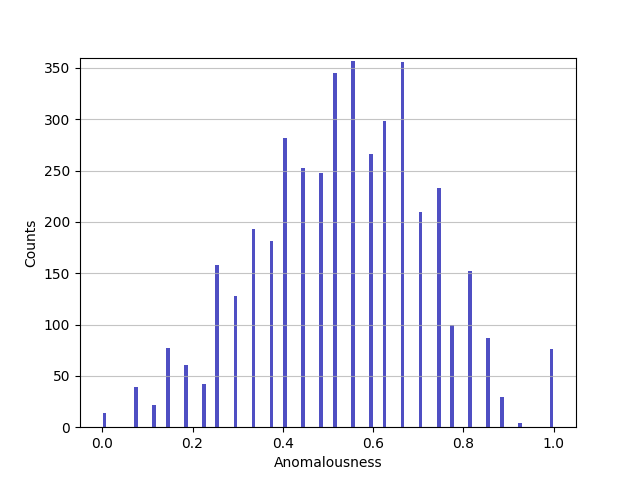
\includegraphics[width=2.5in]{static/spiral_outrank.png}
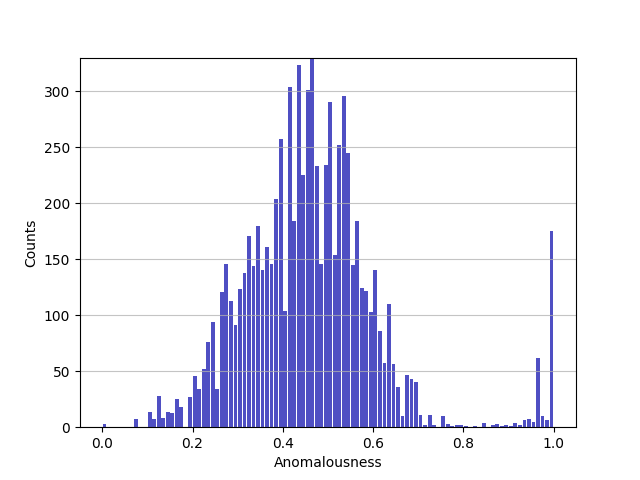
\includegraphics[width=2.5in]{static/interlocking_tori_outrank.png}
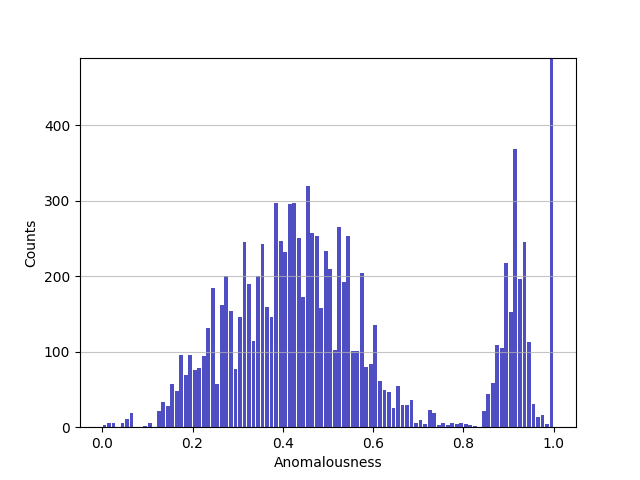
\includegraphics[width=2.5in]{static/skewer_outrank.png}

\caption{
Measures of anomalousness using the Outrank Algorithm on the Bullseye (top-left), Spiral (top-right), Interlocking-Tori (bottom-left), and the Skewer (bottom-right) datasets.
}

\label{results:histograms:outrank}
\end{figure*}


\begin{figure*}[!h]
\centering
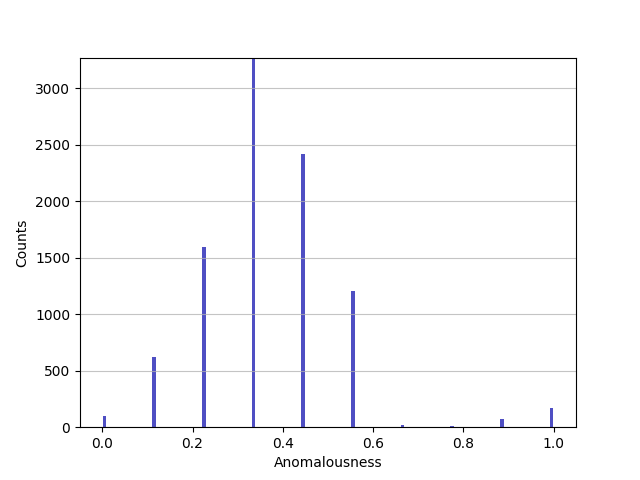
\includegraphics[width=2.5in]{static/bullseye_k_neighborhood.png}
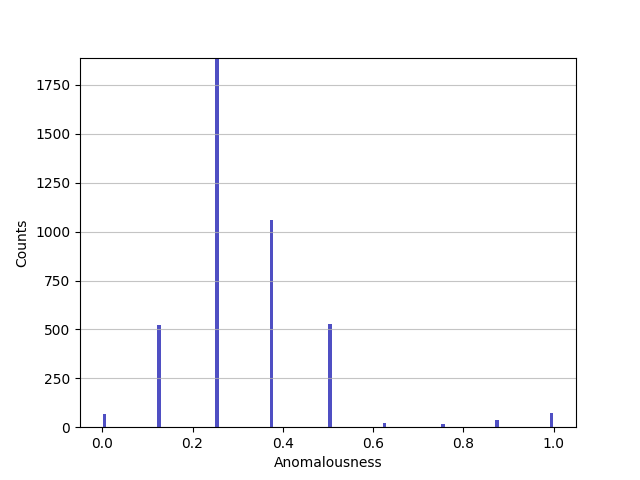
\includegraphics[width=2.5in]{static/spiral_k_neighborhood.png}
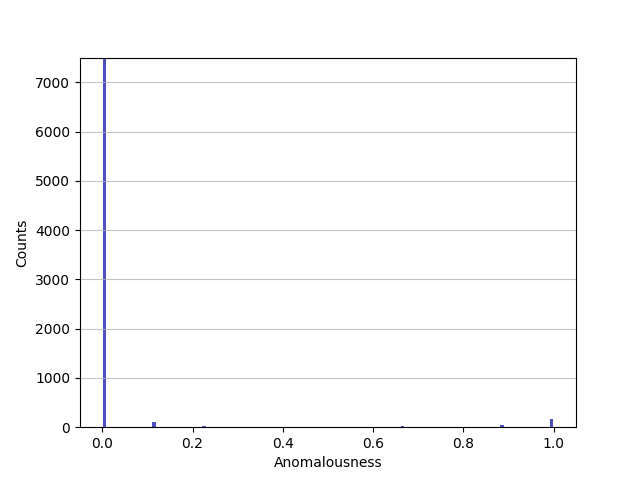
\includegraphics[width=2.5in]{static/interlocking_tori_k_neighborhood.png}
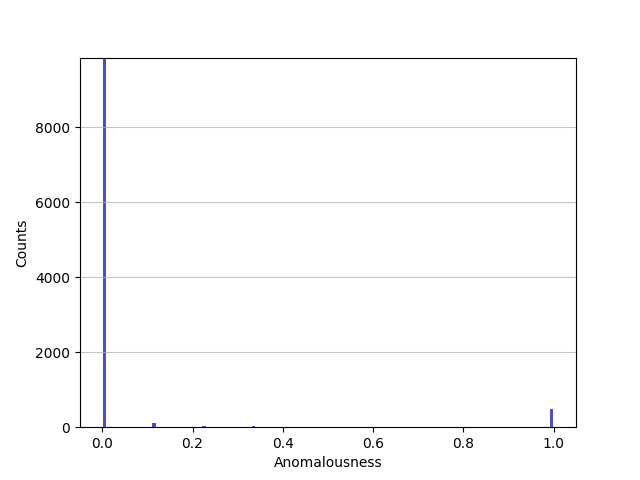
\includegraphics[width=2.5in]{static/skewer_k_neighborhood.png}

\caption{
Measures of anomalousness using the k-Neighborhood Size method on the Bullseye (top-left), Spiral (top-right), Interlocking-Tori (bottom-left), and the Skewer (bottom-right) datasets.
}

\label{results:histograms:k_neighborhood}
\end{figure*}
